% =====================================================================
%  IEEE CONFERENCE PAPER - TOPIC 08: ORDERED TREASURE HUNT
%  Course Project Report: Reinforcement Learning (Fall Semester 2026-2027)
%  Author: Nguyen Duy Hung (Student ID: 24103225)
%  Supervisor: MSc. Vu Hoang Dieu
%  Faculty of Electrical and Electronic Engineering, Phenikaa University
%
%  Format: IEEE Conference 2-Column Template with Official Cover Page
%  Compiler: XeLaTeX or LuaLaTeX (Overleaf compatible)
%  Language: Clear, direct B1-B2 English with exact numerical data
% =====================================================================
\documentclass[10pt,conference]{IEEEtran}
\IEEEoverridecommandlockouts

% Compiler-adaptive font loading
\usepackage{iftex}
\ifXeTeX
  \usepackage{fontspec}
  \setmainfont{TeX Gyre Termes}
  \setsansfont{TeX Gyre Heros}
  \setmonofont{TeX Gyre Cursor}
\else\ifLuaTeX
  \usepackage{fontspec}
  \setmainfont{TeX Gyre Termes}
  \setsansfont{TeX Gyre Heros}
  \setmonofont{TeX Gyre Cursor}
\else
  \usepackage[utf8]{inputenc}
  \usepackage[T1]{fontenc}
  \usepackage{newtxtext,newtxmath}
\fi\fi

\usepackage{cite}
\usepackage{amsmath}
% Prevent clash between amssymb and newtxmath on \Bbbk
\let\Bbbk\relax
\usepackage{amssymb}
\usepackage{amsfonts}
\usepackage{algorithmic}
\usepackage{graphicx}
\usepackage{textcomp}
\usepackage{xcolor}
\usepackage{booktabs}
\usepackage{url}
\usepackage{tikz}
\usetikzlibrary{calc}
\usepackage{multirow}
\usepackage{tabularx}
\usepackage{microtype}

\def\BibTeX{{\rm B\kern-.05em{\sc i\kern-.025em b}\kern-.08em
    T\kern-.1667em\lower.7ex\hbox{E}\kern-.125emX}}

\begin{document}

% =====================================================================
%  COVER PAGE (PAGE 1) - PHENIKAA UNIVERSITY OFFICIAL REPORT FORMAT
% =====================================================================
\begin{titlepage}
\thispagestyle{empty}
\begin{tikzpicture}[remember picture, overlay]

  % Outer Frame Border
  \draw[line width=1.0pt] 
    ($(current page.north west) + (1.23cm, -1.17cm)$) 
    rectangle 
    ($(current page.south east) + (-1.08cm, 1.27cm)$);

  % Topic Box at Top Right
  \node[draw, line width=1.0pt, minimum width=1.1cm, minimum height=1.1cm, anchor=north east] 
    at ($(current page.north east) + (-1.8cm, -1.6cm)$) {
      \fontsize{13}{13}\selectfont\textbf{08}
    };

  % University Header
  \node[anchor=north, align=center] at ($(current page.north) + (0, -3.0cm)$) {
    {\fontsize{13.5}{17}\bfseries PHENIKAA UNIVERSITY}\\[0.25cm]
    {\fontsize{13.5}{17}\bfseries SCHOOL OF ENGINEERING AND TECHNOLOGY}\\[0.25cm]
    {\fontsize{13.5}{17}\bfseries FACULTY OF ELECTRICAL AND ELECTRONIC ENGINEERING}
  };

  % University Logo
  \node[anchor=center] at ($(current page.north) + (0, -7.0cm)$) {
    
\includegraphics[width=3.2cm]{figures/logo_phenikaa.png}
  };

  % Report Subtitle
  \node[anchor=north, align=center] at ($(current page.north) + (0, -9.4cm)$) {
    {\fontsize{12.5}{16}\bfseries COURSE PROJECT REPORT}\\[0.2cm]
    {\fontsize{12.5}{16}\bfseries REINFORCEMENT LEARNING}
  };

  % Project Title
  \node[anchor=north, align=center] at ($(current page.north) + (0, -11.0cm)$) {
    {\fontsize{12.5}{15}\itshape\bfseries Title of the project:}\\[0.35cm]
    {\fontsize{12.5}{16}\bfseries Solving the Ordered Treasure Hunt Problem}\\[0.2cm]
    {\fontsize{12.5}{16}\bfseries in Constrained Gridworlds using Five Tabular}\\[0.2cm]
    {\fontsize{12.5}{16}\bfseries Reinforcement Learning Algorithms}
  };

  % Student and Supervisor Info Table
  \node[anchor=north] at ($(current page.north) + (0, -13.6cm)$) {
    \begin{tabular}{p{2.3cm}p{5.2cm}p{2.5cm}p{5.5cm}}
      \textbf{Student:} & Nguyen Duy Hung & \textbf{Student ID:} & 24103225 \\[0.3cm]
      \textbf{Supervisor:} & MSc. Vu Hoang Dieu & \textbf{Major:} & Electrical and Electronic Engineering
    \end{tabular}
  };

  % Score Box
  \node[draw, line width=0.8pt, minimum width=3.8cm, minimum height=3.2cm, anchor=north] 
    at ($(current page.north) + (0, -15.9cm)$) {};
  \node[anchor=north] at ($(current page.north) + (0, -16.2cm)$) {
    {\fontsize{9}{11}\selectfont Score}
  };

  % Lecturer Signatures Box
  \draw[line width=0.8pt] 
    ($(current page.north) + (-7.2cm, -20.4cm)$) 
    rectangle 
    ($(current page.north) + (7.2cm, -25.0cm)$);
  \draw[line width=0.8pt] 
    ($(current page.north) + (-7.2cm, -21.7cm)$) 
    -- 
    ($(current page.north) + (7.2cm, -21.7cm)$);
  \draw[line width=0.8pt] 
    ($(current page.north) + (0, -20.4cm)$) 
    -- 
    ($(current page.north) + (0, -25.0cm)$);

  \node[anchor=center] at ($(current page.north) + (-3.6cm, -21.05cm)$) {\textbf{Lecturer 1}};
  \node[anchor=center] at ($(current page.north) + (3.6cm, -21.05cm)$) {\textbf{Lecturer 2}};
  \node[anchor=south] at ($(current page.north) + (-3.6cm, -24.5cm)$) {
    {\fontsize{10.5}{13}\selectfont MSc. Vu Hoang Dieu}
  };

  % Location and Date
  \node[anchor=center] at ($(current page.north) + (0, -26.5cm)$) {
    {\fontsize{11.5}{14}\selectfont Hanoi, November 2026}
  };

\end{tikzpicture}
\end{titlepage}

\clearpage
\setcounter{page}{1}

% =====================================================================
%  MAIN PAPER (PAGE 2 ONWARD) - IEEE CONFERENCE TWO-COLUMN FORMAT
% =====================================================================
\title{Solving the Ordered Treasure Hunt Problem in Constrained Gridworlds using Five Tabular Reinforcement Learning Algorithms\thanks{Course Project Report: Reinforcement Learning (Fall Semester 2026--2027), Faculty of Electrical and Electronic Engineering, Phenikaa University, Hanoi, Vietnam.}
}

\author{
  \IEEEauthorblockN{Nguyen Duy Hung}
  \IEEEauthorblockA{
    Student ID: 24103225 \\
    Class: EEE-AI (Artificial Intelligence and Robotics) \\
    Faculty of Electrical and Electronic Engineering, Phenikaa University, Hanoi, Vietnam \\
    Email: 24103225@st.phenikaa-uni.edu.vn
  }
}

\maketitle

\begin{abstract}
In sequential decision-making, an agent must often visit key locations in an exact order before reaching an exit. In this work, we study the Ordered Treasure Hunt problem using tabular reinforcement learning. The agent navigates a gridworld to collect target items in a prescribed sequence. Picking items out of order causes a penalty, and entering the exit door too early is heavily penalized. We design an augmented state vector $s = (r, c, p, w, tok)$ that combines spatial coordinates, task collection progress, a switch flag, and a skip-token flag. We prove mathematically and demonstrate experimentally that tracking task progress inside the state is required to preserve the Markov property. We benchmark five tabular algorithms: Value Iteration, Policy Iteration, Q-Learning, SARSA, and Monte Carlo Control across three square maps ($5\times 5$, $7\times 7$, and $8\times 8$). Across 200 greedy test rollouts, all five algorithms achieve a 100\% mission completion rate. Model-free TD methods find the exact optimal paths discovered by dynamic programming on Level 1 (12 steps) and Level 2 (11 steps). On the hard $8\times 8$ map, we analyze how a bonus shortcut tile creates a local optimum. We also test three step penalty values ($-0.2$, $-1.0$, and $-5.0$), showing how step costs change the optimal collection policy.
\end{abstract}

\begin{IEEEkeywords}
Tabular reinforcement learning, Markov decision process, dynamic programming, Q-learning, SARSA, Monte Carlo control, sequential constraints, gridworld navigation.
\end{IEEEkeywords}

\section{Introduction}
Sequential decision-making under strict ordering constraints is an important challenge in automated systems. In automated warehousing, a mobile robot must collect goods from shelves in a specific order before moving to the packaging station. In robotic assembly, parts must be fitted in an exact mechanical order. If the robot visits the wrong item first, the process fails or requires costly corrections.

In this paper, we study the \textit{Ordered Treasure Hunt} problem using tabular reinforcement learning. The agent moves inside a discrete gridworld. It must collect a set of treasure items in a fixed order, such as $A \rightarrow B \rightarrow C \rightarrow \text{Exit}$. If the agent touches an item out of order or attempts to enter a locked cell, it receives a negative penalty. The exit door opens only after all required items have been collected in the correct order.

A central theoretical question in this problem is state representation. If the state includes only the agent's spatial position $(r, c)$, the environment is not a valid Markov Decision Process (MDP). Entering a cell can produce a positive collection reward if earlier items have been gathered, or a penalty if they have not. Therefore, state transitions and rewards would depend on the past history of the agent. To restore the Markov property, we augment the state into a tuple:
\begin{equation}
    s = (r,\; c,\; p,\; w,\; tok)
\end{equation}
where $r$ and $c$ are grid coordinates, $p$ is the collection progress index, $w$ indicates if a switch is active, and $tok$ tracks whether a bonus skip tile has been used.

We implement and evaluate five foundational tabular algorithms:
\begin{itemize}
    \item \textbf{Value Iteration (VI):} Model-based dynamic programming using the Bellman optimality operator.
    \item \textbf{Policy Iteration (PI):} Model-based dynamic programming alternating policy evaluation and improvement.
    \item \textbf{Q-Learning:} Model-free off-policy Temporal Difference (TD) control.
    \item \textbf{SARSA:} Model-free on-policy Temporal Difference (TD) control.
    \item \textbf{Monte Carlo (MC):} Model-free on-policy first-visit control without bootstrapping.
\end{itemize}

We test all five algorithms across three square maps of increasing difficulty: Level 1 ($5\times 5$, 79 reachable states), Level 2 ($7\times 7$, 199 reachable states), and Level 3 ($8\times 8$, 693 reachable states). The experimental results show that:
\begin{enumerate}
    \item All five algorithms achieve a 100\% mission completion rate across all three maps.
    \item State augmentation with task progress $p$ is strictly necessary to preserve the Markov property.
    \item Model-free TD methods match the exact shortest trajectories found by dynamic programming on Level 1 and Level 2.
    \item On Level 3, the shortcut tile creates a local optimum. Q-Learning escapes this local optimum in 2 out of 3 random seeds, whereas on-policy SARSA and Monte Carlo remain on the shortcut.
    \item Step penalties directly govern policy behavior: cheap steps lead to full item collection, while expensive steps make skipping an item optimal.
\end{enumerate}

\section{Related Work}
Gridworld environments are classic benchmarks in reinforcement learning research \cite{sutton2018reinforcement}. Standard environments such as FrozenLake, Cliff Walking, and Taxi benchmark spatial navigation and obstacle avoidance. However, these standard problems typically have stationary target locations with memoryless state dynamics.

In sequence-constrained problems, the valid next action depends on earlier accomplishments. When the state space does not capture this history, the environment becomes a Partially Observable Markov Decision Process (POMDP) \cite{bertsekas2012dynamic}. Researchers have addressed sequence constraints by adding memory variables or using finite-state automata \cite{watkins1992q, rummery1994line}. In tabular reinforcement learning, the cleanest and most rigorous solution is explicit state augmentation. By appending discrete task progress variables to the spatial coordinates, the augmented state satisfies the Markov property while keeping the total number of states small enough for exact tabular storage.

\section{Problem Formulation}

\subsection{Environment Description}
The Ordered Treasure Hunt environment is a discrete 2D gridworld. The agent moves in four cardinal directions: $\mathcal{A} = \{\text{Up}, \text{Down}, \text{Left}, \text{Right}\}$. Moving into a wall or the outer boundary keeps the agent in place and incurs a collision penalty. Table~\ref{tab:symbols} defines the ASCII map symbols.

\begin{table}[htbp]
\caption{Map Symbol Specifications}
\label{tab:symbols}
\centering
\begin{tabular}{cll}
\toprule
\textbf{Symbol} & \textbf{Entity} & \textbf{Semantics} \\
\midrule
\texttt{\#} & Wall & Impassable obstacle; causes bounce and penalty \\
\texttt{.} & Floor & Walkable open corridor \\
\texttt{S} & Start & Initial position of the agent $(r_0, c_0)$ \\
\texttt{A, B, C, D} & Targets & Items that must be collected in sequence \\
\texttt{W} & Switch & Activation lever that unlocks locked target \texttt{C} \\
\texttt{K} & Skip Tile & Bonus tile that advances sequence progress by 1 \\
\texttt{E} & Exit & Goal cell; opens only when sequence is complete \\
\bottomrule
\end{tabular}
\end{table}

\subsection{Benchmark Configurations}
We evaluate three benchmark maps with increasing spatial and logical complexity (Fig.~\ref{fig:maps} and Table~\ref{tab:configs}):
\begin{itemize}
    \item \textbf{Level 1: Easy ($5\times 5$):} A single chain $A \rightarrow B \rightarrow C \rightarrow \text{Exit}$. It contains 22 walkable cells and 79 reachable states.
    \item \textbf{Level 2: Medium ($7\times 7$):} A branching layout offering two valid chains: $A \rightarrow B \rightarrow D$ or $A \rightarrow C \rightarrow D$. It contains 36 walkable cells and 199 reachable states.
    \item \textbf{Level 3: Hard ($8\times 8$):} A 4-item chain $A \rightarrow B \rightarrow C \rightarrow D$. Target $C$ is locked behind switch $W$. A bonus tile $K$ allows skipping one item. It contains 49 walkable cells and 693 reachable states.
\end{itemize}

\begin{figure*}[htbp]
\centering
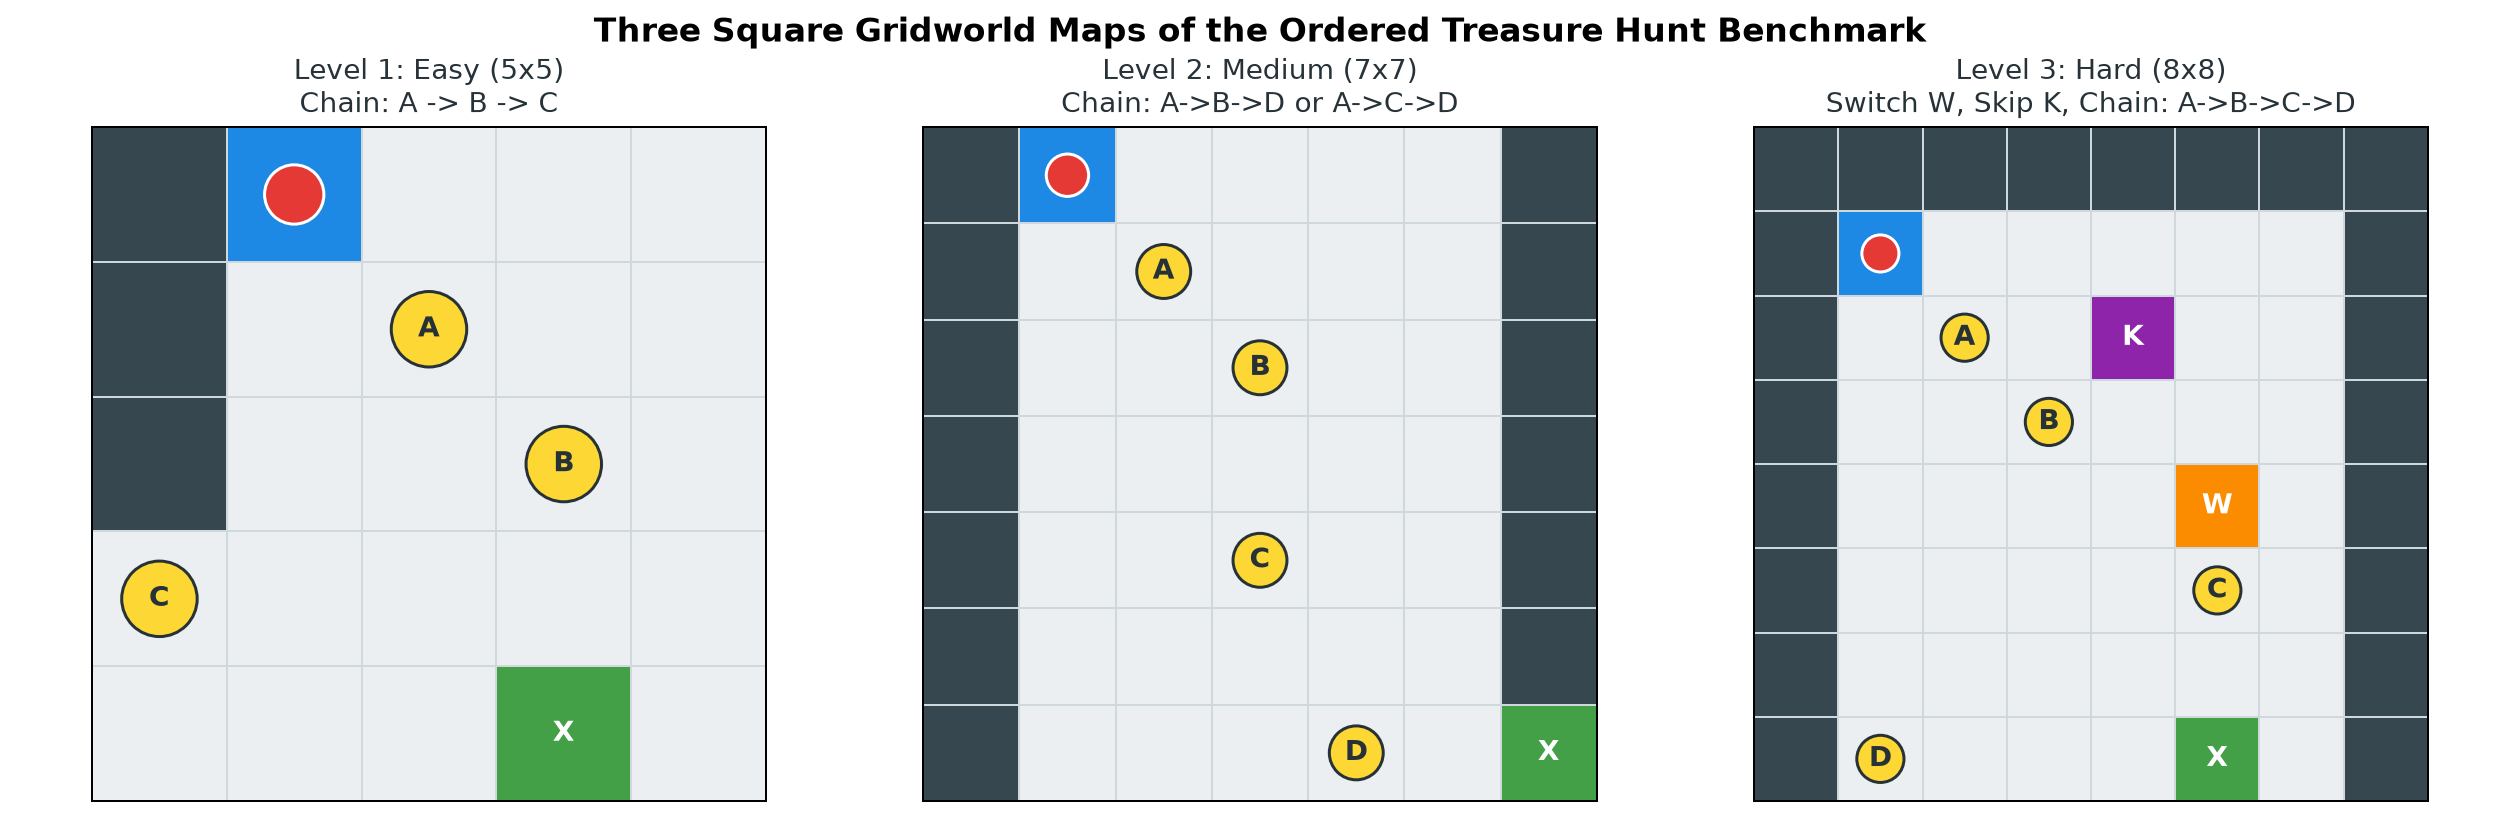
\includegraphics[width=0.92\textwidth]{figures/env_levels.png}
\caption{The three benchmark gridworld maps: Level 1 ($5\times 5$, single chain $A \rightarrow B \rightarrow C$), Level 2 ($7\times 7$, two valid branches), and Level 3 ($8\times 8$, locked item $C$, switch $W$, and skip tile $K$).}
\label{fig:maps}
\end{figure*}

\begin{table}[htbp]
\caption{Configuration Properties of Benchmark Maps}
\label{tab:configs}
\centering
\begin{tabular}{lccccc}
\toprule
\textbf{Map} & \textbf{Grid} & \textbf{Walkable} & $\mathbf{|\mathcal{S}|}$ & $\mathbf{|\mathcal{A}|}$ & \textbf{Required Sequence} \\
\midrule
Level 1: Easy   & $5 \times 5$ & 22 & 79  & 4 & $A \rightarrow B \rightarrow C \rightarrow \text{Exit}$ \\
Level 2: Medium & $7 \times 7$ & 36 & 199 & 4 & $A \rightarrow (B \text{ or } C) \rightarrow D \rightarrow \text{Exit}$ \\
Level 3: Hard   & $8 \times 8$ & 49 & 693 & 4 & $A \rightarrow B \rightarrow C \rightarrow D \rightarrow \text{Exit}$ \\
\bottomrule
\end{tabular}
\end{table}

\subsection{State Representation and Markov Property Proof}
A stochastic process possesses the Markov property if the conditional probability distribution of future states depends solely on the current state and action:
\begin{equation}
    P(s_{t+1} \mid s_t, a_t, s_{t-1}, a_{t-1}, \dots, s_0, a_0) = P(s_{t+1} \mid s_t, a_t)
\end{equation}

If the state consists only of grid coordinates $(r, c)$, this property is violated. Consider cell $(2, 1)$ on Level 1 (Fig.~\ref{fig:markov}). If the agent moves Right to $(2, 2)$:
\begin{itemize}
    \item When the agent has not yet collected item $A$ ($p = 0$), target $A$ is present. The agent collects item $A$, receiving $r = +10.0$ and advancing progress to $p = 1$.
    \item When the agent has already collected item $A$ ($p = 1$), target $A$ is no longer on the board. The same move to $(2, 2)$ lands on an empty floor, yielding step penalty $r = -1.0$.
\end{itemize}

\begin{figure}[htbp]
\centering
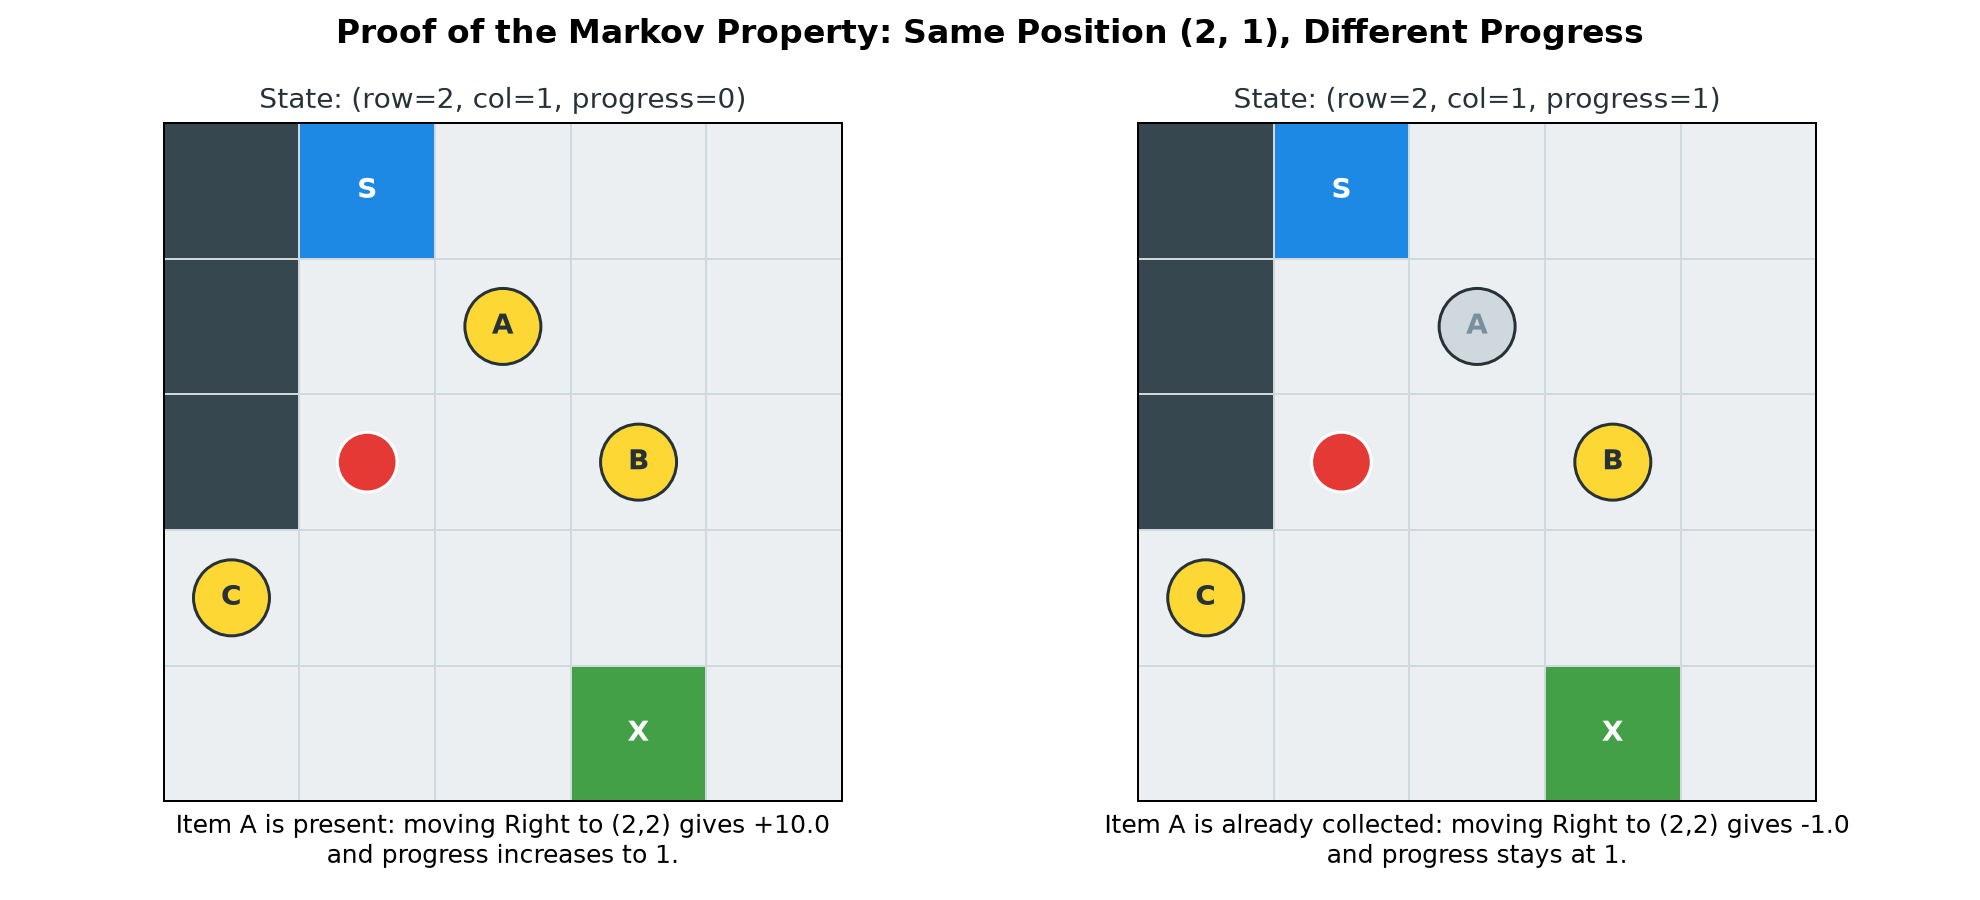
\includegraphics[width=0.48\textwidth]{figures/markov_proof.png}
\caption{Proof of the Markov property at cell $(2, 1)$ on Level 1. When $p=0$ (left), moving right collects item $A$ (+10.0). When $p=1$ (right), item $A$ is already taken, yielding step cost (-1.0). Progress $p$ must be in the state.}
\label{fig:markov}
\end{figure}

Without progress $p$, the reward and transition functions cannot be evaluated without knowing past actions. Therefore, we define the state vector as:
\begin{equation}
    s = (r,\; c,\; p,\; w,\; tok)
\end{equation}
where $r \in [0, H-1]$, $c \in [0, W-1]$, $p \in [0, N_{\text{stages}}]$, $w \in \{0, 1\}$, and $tok \in \{0, 1\}$. With this state vector, all transitions and rewards are stationary and memoryless.

\subsection{Reward Formulation and Early-Exit Prevention}
The reward function is formulated to guide efficient navigation while penalizing improper actions (Table~\ref{tab:rewards}):
\begin{equation}
    R(s, a, s') = 
    \begin{cases}
        r_{\text{exit}} = +100.0, & \text{if exit reached with task complete} \\
        r_{\text{collect}} = +10.0, & \text{if correct next target is collected} \\
        r_{\text{early}} = -20.0, & \text{if exit entered prematurely} \\
        r_{\text{wrong}} = -20.0, & \text{if touching out-of-order target} \\
        r_{\text{wall}} = -3.0, & \text{if colliding with wall} \\
        r_{\text{step}} = -1.0, & \text{for standard floor movement}
    \end{cases}
\end{equation}

\begin{table}[htbp]
\caption{Baseline Reward Formulation Specifications}
\label{tab:rewards}
\centering
\begin{tabular}{lrl}
\toprule
\textbf{Reward Parameter} & \textbf{Value} & \textbf{Design Purpose} \\
\midrule
Step penalty $r_{\text{step}}$ & $-1.0$ & Encourages shortest path navigation \\
Wall penalty $r_{\text{wall}}$ & $-3.0$ & Prevents unnecessary boundary collisions \\
Target reward $r_{\text{collect}}$ & $+10.0$ & Encourages sequence progression \\
Wrong item penalty $r_{\text{wrong}}$ & $-20.0$ & Punishes out-of-order visits \\
Exit bonus $r_{\text{exit}}$ & $+100.0$ & Goal completion incentive \\
Early exit penalty $r_{\text{early}}$ & $-20.0$ & Prevents quitting before completion \\
\bottomrule
\end{tabular}
\end{table}

A critical detail is the premature exit penalty $r_{\text{early}} = -20.0$. If entering the exit early incurred no penalty or simply ended the episode, an exploratory agent would quickly terminate at the exit door to avoid cumulative step penalties. By assigning a large negative penalty $r_{\text{early}} = -20.0$, the agent learns to avoid the exit until the entire item chain is completed.

\subsection{Termination and Horizon Truncation}
An episode terminates under two conditions:
\begin{enumerate}
    \item \textbf{Terminal Success:} The agent reaches the exit cell after collecting all required items in the correct order. At this state, $V(s_{\text{term}}) = 0$.
    \item \textbf{Horizon Truncation:} The elapsed steps reach $H = 100$. Truncation stops infinite wandering during early exploration. Because truncation is not a true terminal state, bootstrapping must not artificially zero out value updates.
\end{enumerate}

\section{The Five Tabular RL Algorithms}

\subsection{Dynamic Programming Methods (Model-Based)}
Dynamic programming methods require explicit knowledge of the transition probability tensor $\mathcal{P}(s' \mid s, a)$ and reward matrix $\mathcal{R}(s, a)$. The environment builds these models by forward state expansion.

\textbf{1) Value Iteration (VI):} Iteratively applies the Bellman optimality backup across all states:
\begin{equation}
    V_{k+1}(s) = \max_{a \in \mathcal{A}} \left[ \mathcal{R}(s, a) + \gamma \sum_{s' \in \mathcal{S}} \mathcal{P}(s' \mid s, a) V_k(s') \right]
\end{equation}
The algorithm terminates when the maximum value change falls below $\theta = 10^{-8}$:
\begin{equation}
    \max_{s \in \mathcal{S}} |V_{k+1}(s) - V_k(s)| < \theta
\end{equation}
The greedy policy is then extracted via:
\begin{equation}
    \pi^*(s) = \arg\max_{a \in \mathcal{A}} \left[ \mathcal{R}(s, a) + \gamma \sum_{s' \in \mathcal{S}} \mathcal{P}(s' \mid s, a) V^*(s') \right]
\end{equation}

\textbf{2) Policy Iteration (PI):} Alternates between exact policy evaluation and policy improvement. Policy evaluation solves the linear Bellman equation until $\Delta < 10^{-8}$:
\begin{equation}
    V^\pi(s) = \mathcal{R}(s, \pi(s)) + \gamma \sum_{s' \in \mathcal{S}} \mathcal{P}(s' \mid s, \pi(s)) V^\pi(s')
\end{equation}
Policy improvement updates the action at each state:
\begin{equation}
    \pi_{\text{new}}(s) = \arg\max_{a \in \mathcal{A}} \left[ \mathcal{R}(s, a) + \gamma \sum_{s' \in \mathcal{S}} \mathcal{P}(s' \mid s, a) V^\pi(s') \right]
\end{equation}
The process halts when $\pi_{\text{new}}(s) = \pi(s)$ for all $s \in \mathcal{S}$.

\subsection{Temporal Difference Learning Methods (Model-Free)}
Model-free TD algorithms learn action-value tables $Q(s, a)$ from experienced transition samples $(s_t, a_t, r_{t+1}, s_{t+1})$ without model knowledge.

\textbf{3) Q-Learning (Off-Policy TD):} Updates action values using the greedy target:
\begin{equation}
    Q(s_t, a_t) \leftarrow Q(s_t, a_t) + \alpha \left[ r_{t+1} + \gamma \max_{a'} Q(s_{t+1}, a') - Q(s_t, a_t) \right]
\end{equation}
Because the update uses $\max_{a'}$, Q-learning directly estimates the optimal action values $Q^*(s, a)$ regardless of the action selected by the exploration policy.

\textbf{4) SARSA (On-Policy TD):} Updates action values using the next action $a_{t+1}$ chosen by the current $\epsilon$-greedy policy:
\begin{equation}
    Q(s_t, a_t) \leftarrow Q(s_t, a_t) + \alpha \left[ r_{t+1} + \gamma Q(s_{t+1}, a_{t+1}) - Q(s_t, a_t) \right]
\end{equation}
Because SARSA accounts for exploratory actions taken by the behavior policy, it learns safer trajectories near high-penalty areas.

\subsection{Monte Carlo Control (Model-Free, Non-Bootstrapped)}
\textbf{5) Monte Carlo Control (MC):} Gathers complete trajectory rollouts before performing updates. For each episode, it computes the discounted return from step $t$:
\begin{equation}
    G_t = \sum_{k=t}^T \gamma^{k-t} r_{k+1}
\end{equation}
Using first-visit tracking, it updates the state-action values with learning rate $\alpha$:
\begin{equation}
    Q(s_t, a_t) \leftarrow Q(s_t, a_t) + \alpha \left[ G_t - Q(s_t, a_t) \right]
\end{equation}
Monte Carlo control does not bootstrap, making it unbiased but subject to higher return variance.

\subsection{Architectural Comparison}
Table~\ref{tab:algo_arch} compares the architectural features of the five algorithms.

\begin{table}[htbp]
\caption{Architectural Comparison of the Five RL Algorithms}
\label{tab:algo_arch}
\centering
\begin{tabular}{lcccc}
\toprule
\textbf{Algorithm} & \textbf{Model} & \textbf{Policy Type} & \textbf{Bootstrap} & \textbf{Update Target} \\
\midrule
Value Iteration    & Required & Off-policy & Yes & Bellman optimality \\
Policy Iteration   & Required & Off-policy & Yes & Policy evaluation \\
Q-Learning         & Free     & Off-policy & Yes & $r + \gamma \max_{a'} Q(s', a')$ \\
SARSA              & Free     & On-policy  & Yes & $r + \gamma Q(s', a')$ \\
Monte Carlo        & Free     & On-policy  & No  & Complete return $G_t$ \\
\bottomrule
\end{tabular}
\end{table}

\section{Experimental Design}

\subsection{Hyperparameter Settings}
Table~\ref{tab:hyperparams} lists the global hyperparameter specifications. Model-free agents train for 20,000 episodes with an exploration rate $\epsilon$ decaying linearly from 1.0 to 0.05. The discount factor is $\gamma = 0.99$, and the learning rate is $\alpha = 0.1$. Dynamic programming methods use convergence threshold $\theta = 10^{-8}$.

\begin{table}[htbp]
\caption{Global Hyperparameter Specifications}
\label{tab:hyperparams}
\centering
\begin{tabular}{lrl}
\toprule
\textbf{Hyperparameter} & \textbf{Value} & \textbf{Description} \\
\midrule
Training episodes & 20,000 & Total training rollouts for TD and MC \\
Evaluation rollouts & 200 & Deterministic evaluation rollouts ($\epsilon = 0$) \\
Discount factor $\gamma$ & 0.99 & Discounting for future rewards \\
Learning rate $\alpha$ & 0.10 & Step size for TD and MC updates \\
Exploration $\epsilon_{\text{start}}$ & 1.00 & Initial exploration probability \\
Exploration $\epsilon_{\text{end}}$ & 0.05 & Final exploration probability floor \\
$\epsilon$ schedule & Linear & Decayed across all 20,000 episodes \\
DP threshold $\theta$ & $10^{-8}$ & Stopping criterion for VI and PI \\
Horizon limit $H$ & 100 & Maximum steps per episode \\
Evaluation $\epsilon$ & 0.00 & Purely greedy policy execution \\
Random seed & 42 & Base seed (with 7, 123 for seed tests) \\
\bottomrule
\end{tabular}
\end{table}

\subsection{Evaluation Protocols}
Following training, each model-free policy is evaluated greedily ($\epsilon = 0$) over 200 rollouts. We record four primary metrics:
\begin{itemize}
    \item \textbf{Mean Undiscounted Return:} Total sum of step rewards accumulated in an evaluation episode.
    \item \textbf{Path Length (Steps):} Total steps taken from start to the exit door.
    \item \textbf{Success Rate (\%):} Fraction of evaluation episodes completing the task within 100 steps.
    \item \textbf{Computation Time (s):} Total wall-clock time required for training and policy extraction.
\end{itemize}

\section{Experimental Results}

\subsection{Dynamic Programming Reference Solutions}
Table~\ref{tab:dp_results} presents the exact ground-truth solutions produced by Value Iteration and Policy Iteration. Both algorithms find the exact same optimal paths: 12 steps on Level 1, 11 steps on Level 2, and 18 steps on Level 3. Policy Iteration converges in fewer iterations (4 to 9 policy evaluations) than Value Iteration (16 to 26 sweeps), although each policy evaluation involves solving a system of equations.

\begin{table}[htbp]
\caption{Dynamic Programming Benchmark Results}
\label{tab:dp_results}
\centering
\begin{tabular}{llccccc}
\toprule
\textbf{Map} & \textbf{Algorithm} & \textbf{Return} & \textbf{Steps} & \textbf{Success} & \textbf{Time (s)} & \textbf{Iter.} \\
\midrule
Level 1 & Value Iteration  & $+122.0$ & 12.0 & 100\% & 0.0024 & 16 \\
Level 1 & Policy Iteration & $+122.0$ & 12.0 & 100\% & 0.1441 & 4  \\
\midrule
Level 2 & Value Iteration  & $+123.0$ & 11.0 & 100\% & 0.0064 & 18 \\
Level 2 & Policy Iteration & $+123.0$ & 11.0 & 100\% & 0.6459 & 6  \\
\midrule
Level 3 & Value Iteration  & $+128.0$ & 18.0 & 100\% & 0.0354 & 26 \\
Level 3 & Policy Iteration & $+128.0$ & 18.0 & 100\% & 3.7050 & 9  \\
\bottomrule
\end{tabular}
\end{table}

\subsection{Performance of Model-Free Algorithms}
Table~\ref{tab:modelfree_results} summarizes the performance of all five algorithms across the three benchmark maps. All five algorithms achieve a 100\% mission completion rate.

\begin{table}[htbp]
\caption{Comprehensive Benchmark Performance Across All Maps}
\label{tab:modelfree_results}
\centering
\begin{tabular}{llcccc}
\toprule
\textbf{Map} & \textbf{Algorithm} & \textbf{Return} & \textbf{Steps} & \textbf{Success} & \textbf{Time (s)} \\
\midrule
Level 1 & Value Iteration  & $+122.0$ & 12.0 & 100\% & 0.002 \\
Level 1 & Policy Iteration & $+122.0$ & 12.0 & 100\% & 0.144 \\
Level 1 & Q-Learning       & $+122.0$ & 12.0 & 100\% & 8.985 \\
Level 1 & SARSA            & $+122.0$ & 12.0 & 100\% & 9.756 \\
Level 1 & Monte Carlo      & $+122.0$ & 12.0 & 100\% & 6.409 \\
\midrule
Level 2 & Value Iteration  & $+123.0$ & 11.0 & 100\% & 0.006 \\
Level 2 & Policy Iteration & $+123.0$ & 11.0 & 100\% & 0.646 \\
Level 2 & Q-Learning       & $+123.0$ & 11.0 & 100\% & 8.544 \\
Level 2 & SARSA            & $+123.0$ & 11.0 & 100\% & 9.694 \\
Level 2 & Monte Carlo      & $+123.0$ & 11.0 & 100\% & 6.051 \\
\midrule
Level 3 & Value Iteration  & $+128.0$ & 18.0 & 100\% & 0.035 \\
Level 3 & Policy Iteration & $+128.0$ & 18.0 & 100\% & 3.705 \\
Level 3 & Q-Learning       & $+120.0$ & 18.0 & 100\% & 27.069 \\
Level 3 & SARSA            & $+120.0$ & 18.0 & 100\% & 14.515 \\
Level 3 & Monte Carlo      & $+119.0$ & 18.0 & 100\% & 9.599 \\
\bottomrule
\end{tabular}
\end{table}

On Level 1, all five algorithms converge to the analytical optimum: $+122.0$ return in exactly 12 steps. On Level 2, all agents find the optimal 11-step path ($+123.0$), correctly choosing the shorter branch ($A \rightarrow B \rightarrow D$) over the longer alternate route. On Level 3, dynamic programming identifies the 18-step full sequence route earning $+128.0$. Under baseline seed 42, the model-free methods converge to 18 steps with returns of $+119.0$ to $+120.0$, utilizing the bonus skip tile $K$.

\subsection{Learning Dynamics and Convergence}
Fig.~\ref{fig:curves} illustrates the training return curves of Q-Learning across the three levels. On Level 1 ($5\times 5$), the agent learns the task rapidly, reaching steady-state performance within 300 episodes. On Level 2 ($7\times 7$), the agent reaches full task competency within roughly 800 episodes. On Level 3 ($8\times 8$), the larger state space ($|\mathcal{S}| = 693$) and additional mechanisms (switch $W$ and skip tile $K$) require roughly 1,500 episodes before reaching steady high returns.

\begin{figure}[htbp]
\centering
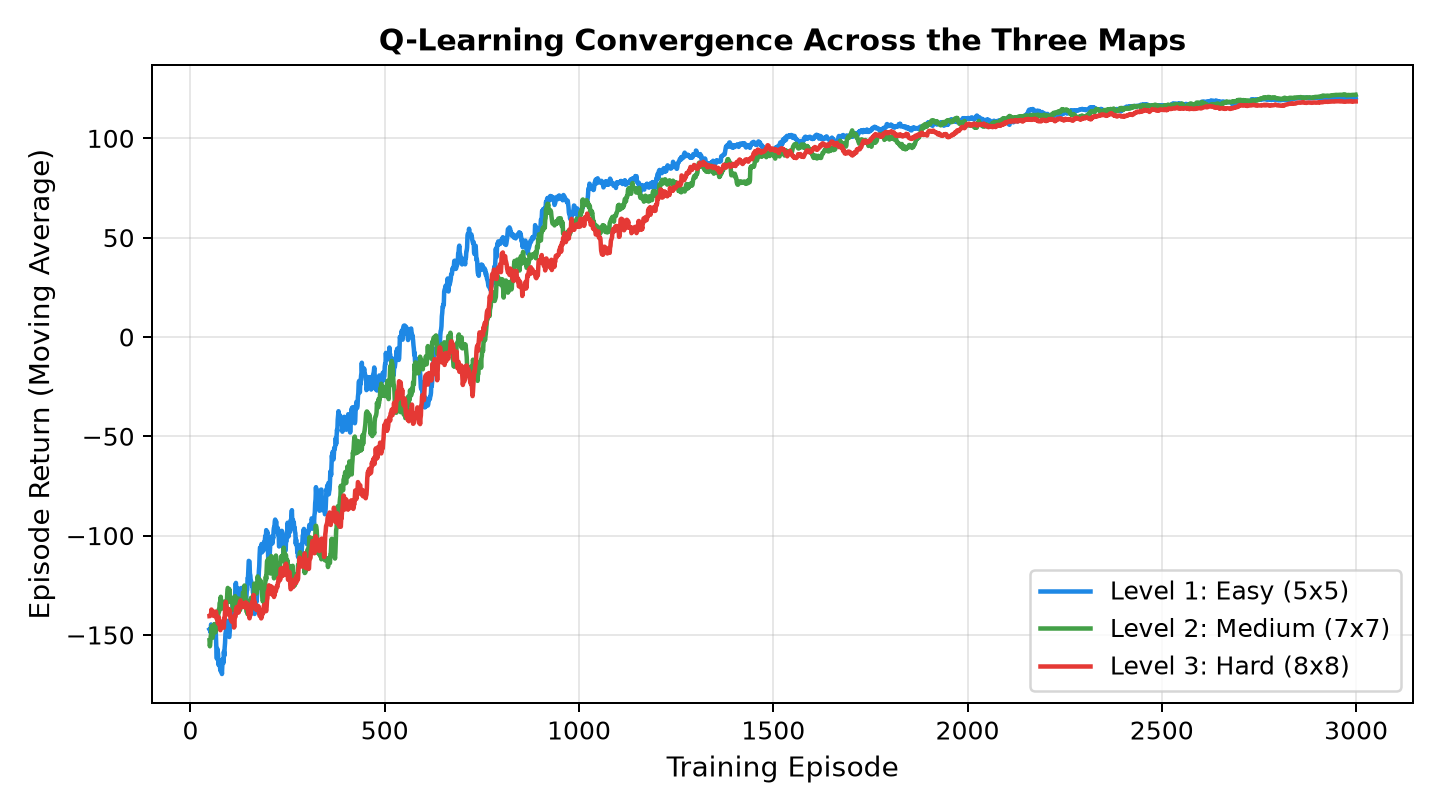
\includegraphics[width=0.48\textwidth]{figures/learning_curves.png}
\caption{Learning curves of Q-Learning over 3,000 training episodes across Level 1, Level 2, and Level 3.}
\label{fig:curves}
\end{figure}

\subsection{Trajectory and Policy Visualizations}
Fig.~\ref{fig:trajectories} visualizes the optimal trajectories discovered on the three benchmark maps. The agent navigates efficiently between targets while avoiding locked cells and boundary walls.

\begin{figure*}[htbp]
\centering
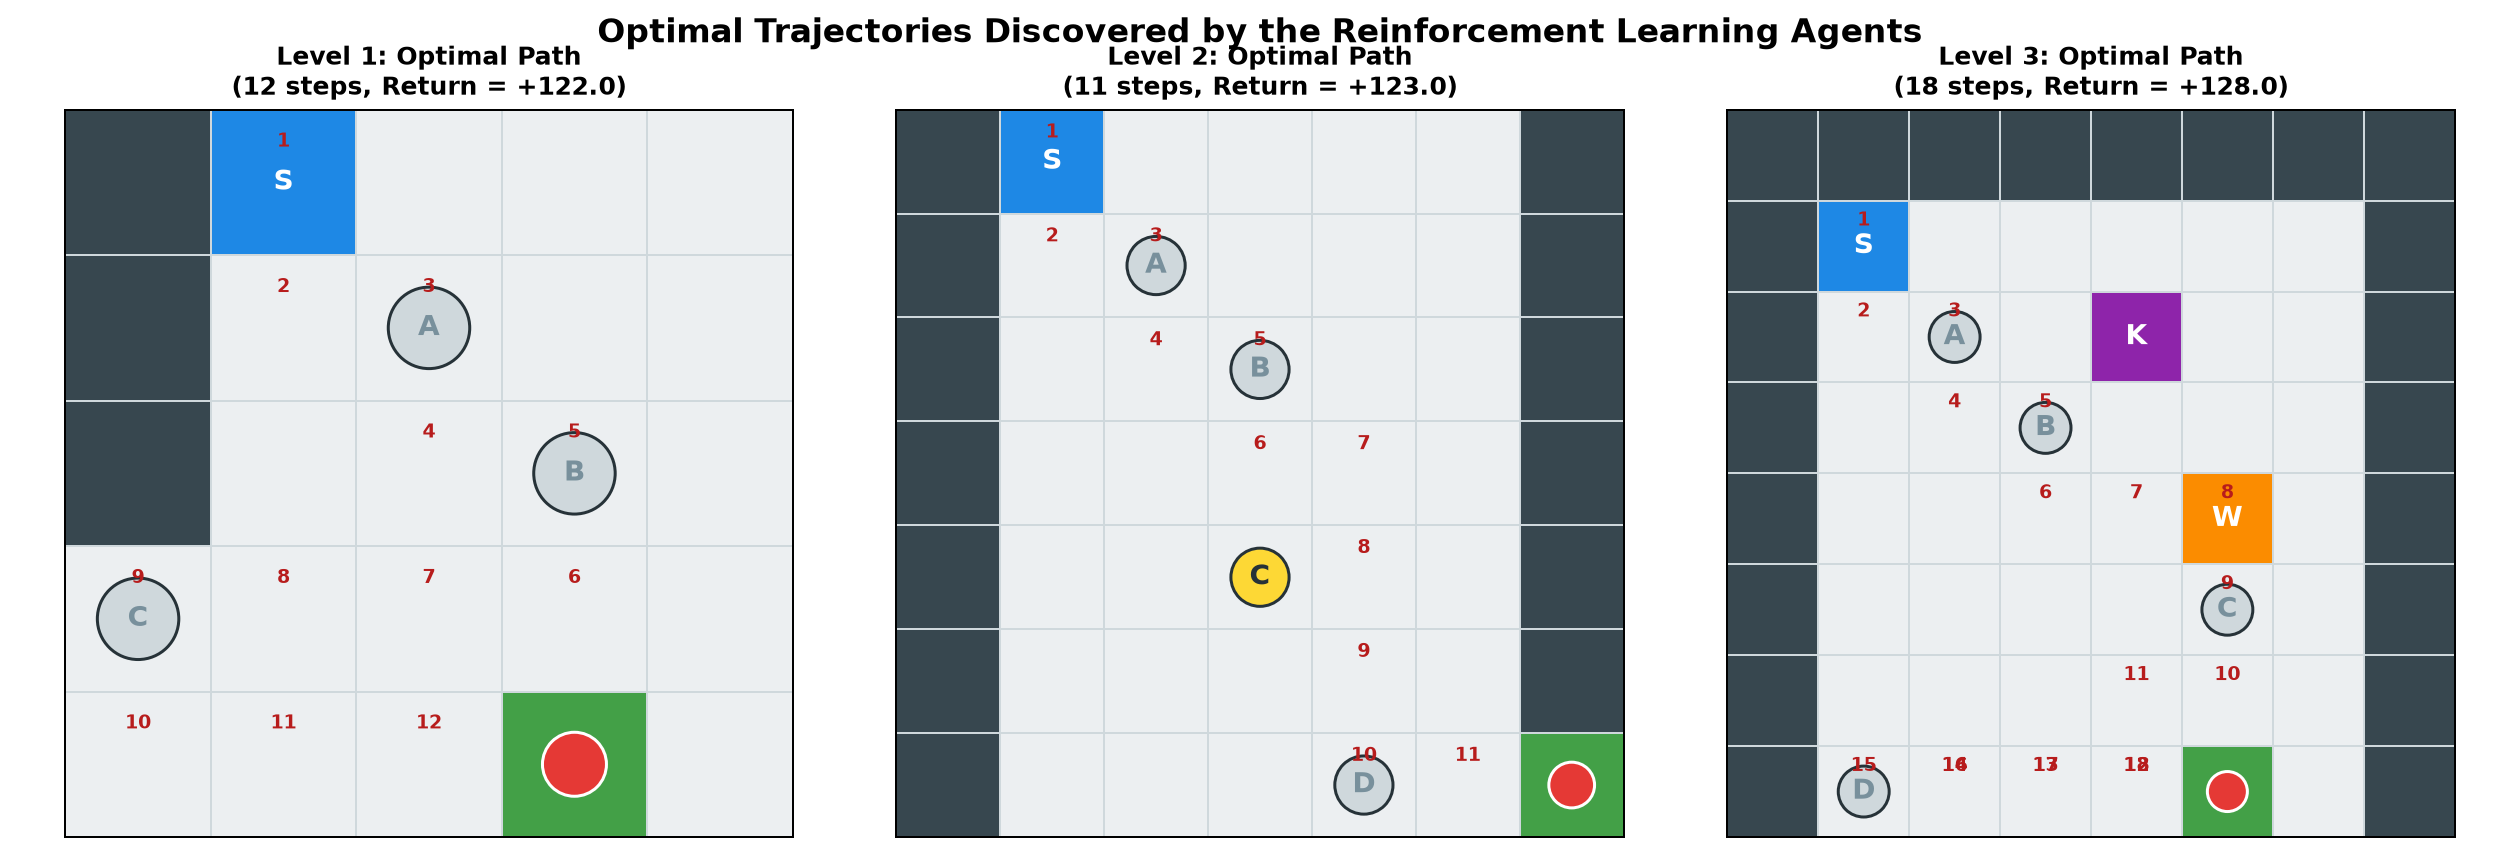
\includegraphics[width=0.92\textwidth]{figures/optimal_paths.png}
\caption{Optimal navigation trajectories: Level 1 (12 steps, $A \rightarrow B \rightarrow C$), Level 2 (11 steps, shorter branch $A \rightarrow B \rightarrow D$), and Level 3 (18 steps, full sequence $A \rightarrow W \rightarrow C \rightarrow D$).}
\label{fig:trajectories}
\end{figure*}

Fig.~\ref{fig:policies} shows the extracted greedy policy action grids on Level 1, Level 2, and Level 3. Arrows indicate the optimal movement direction at each cell.

\begin{figure*}[htbp]
\centering
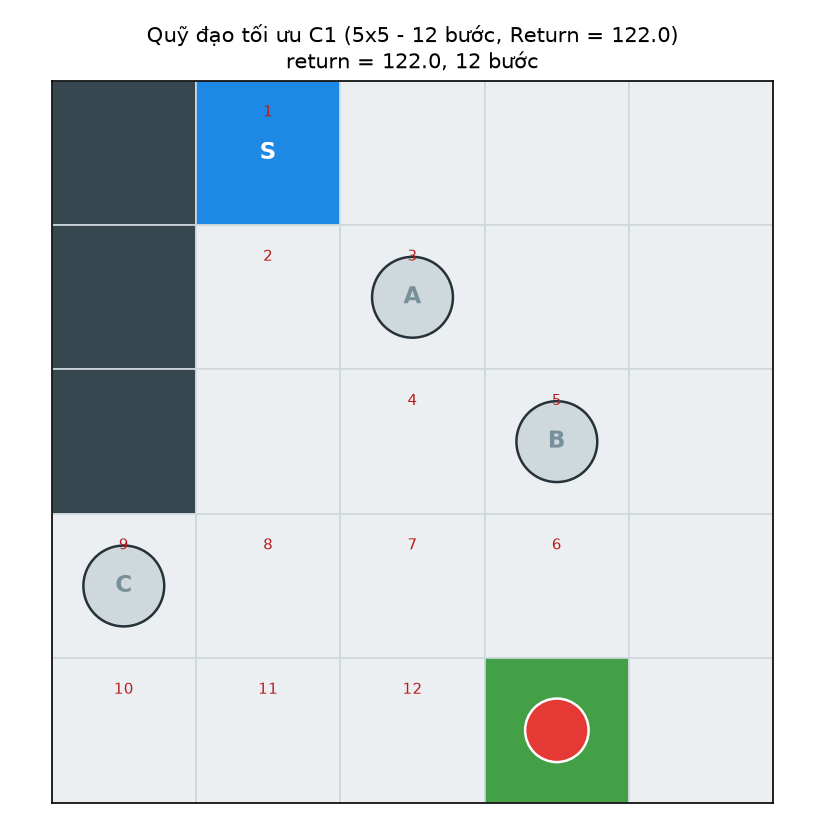
\includegraphics[width=0.31\textwidth]{figures/policy_C1_Easy_5x5.png} \hfill
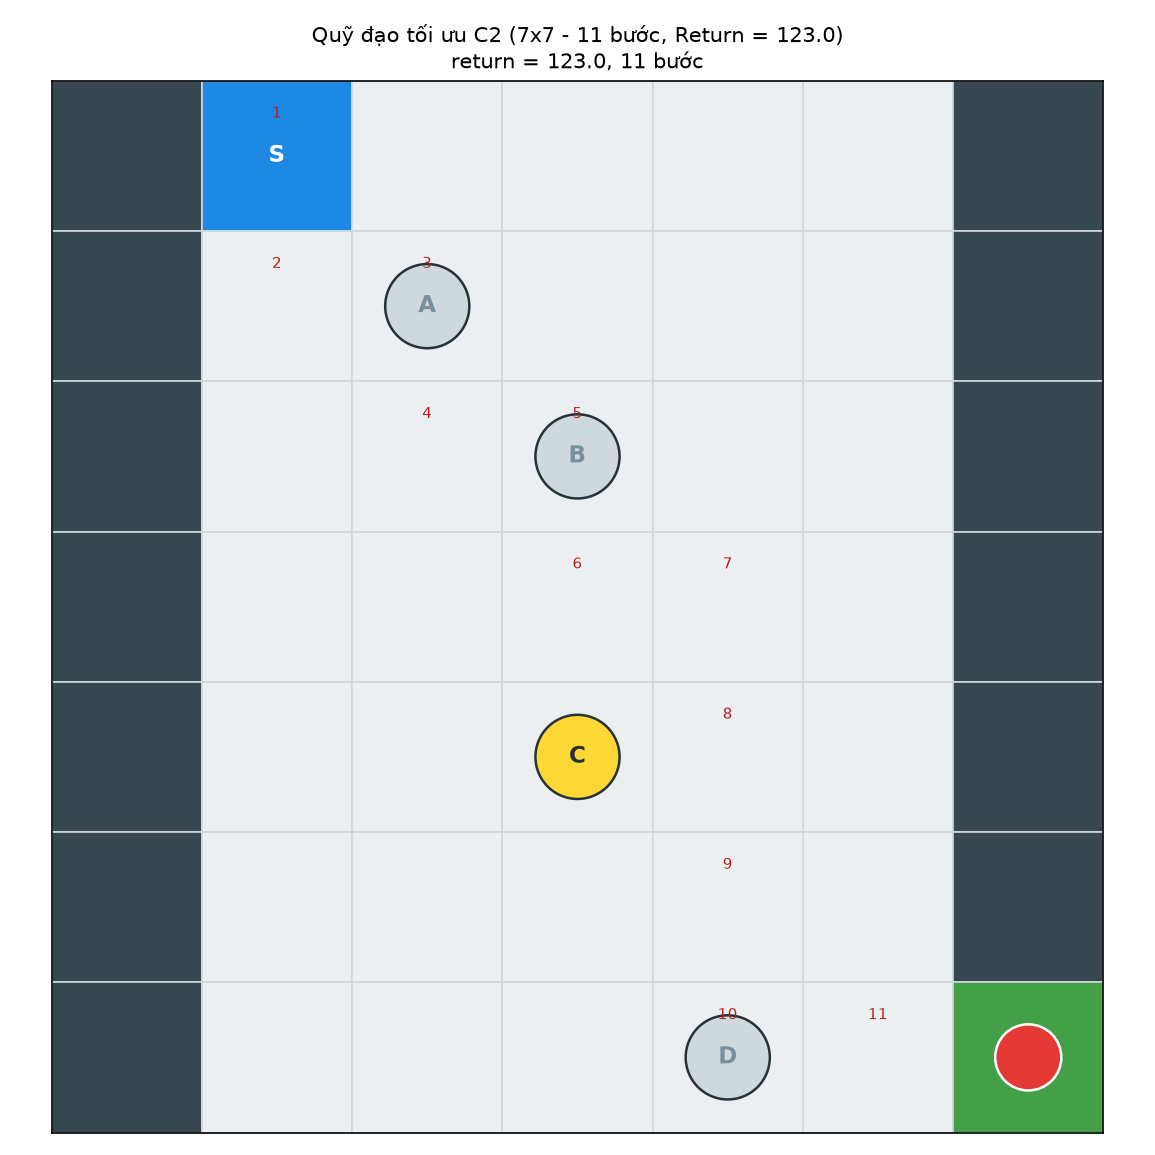
\includegraphics[width=0.31\textwidth]{figures/policy_C2_Medium_7x7.png} \hfill
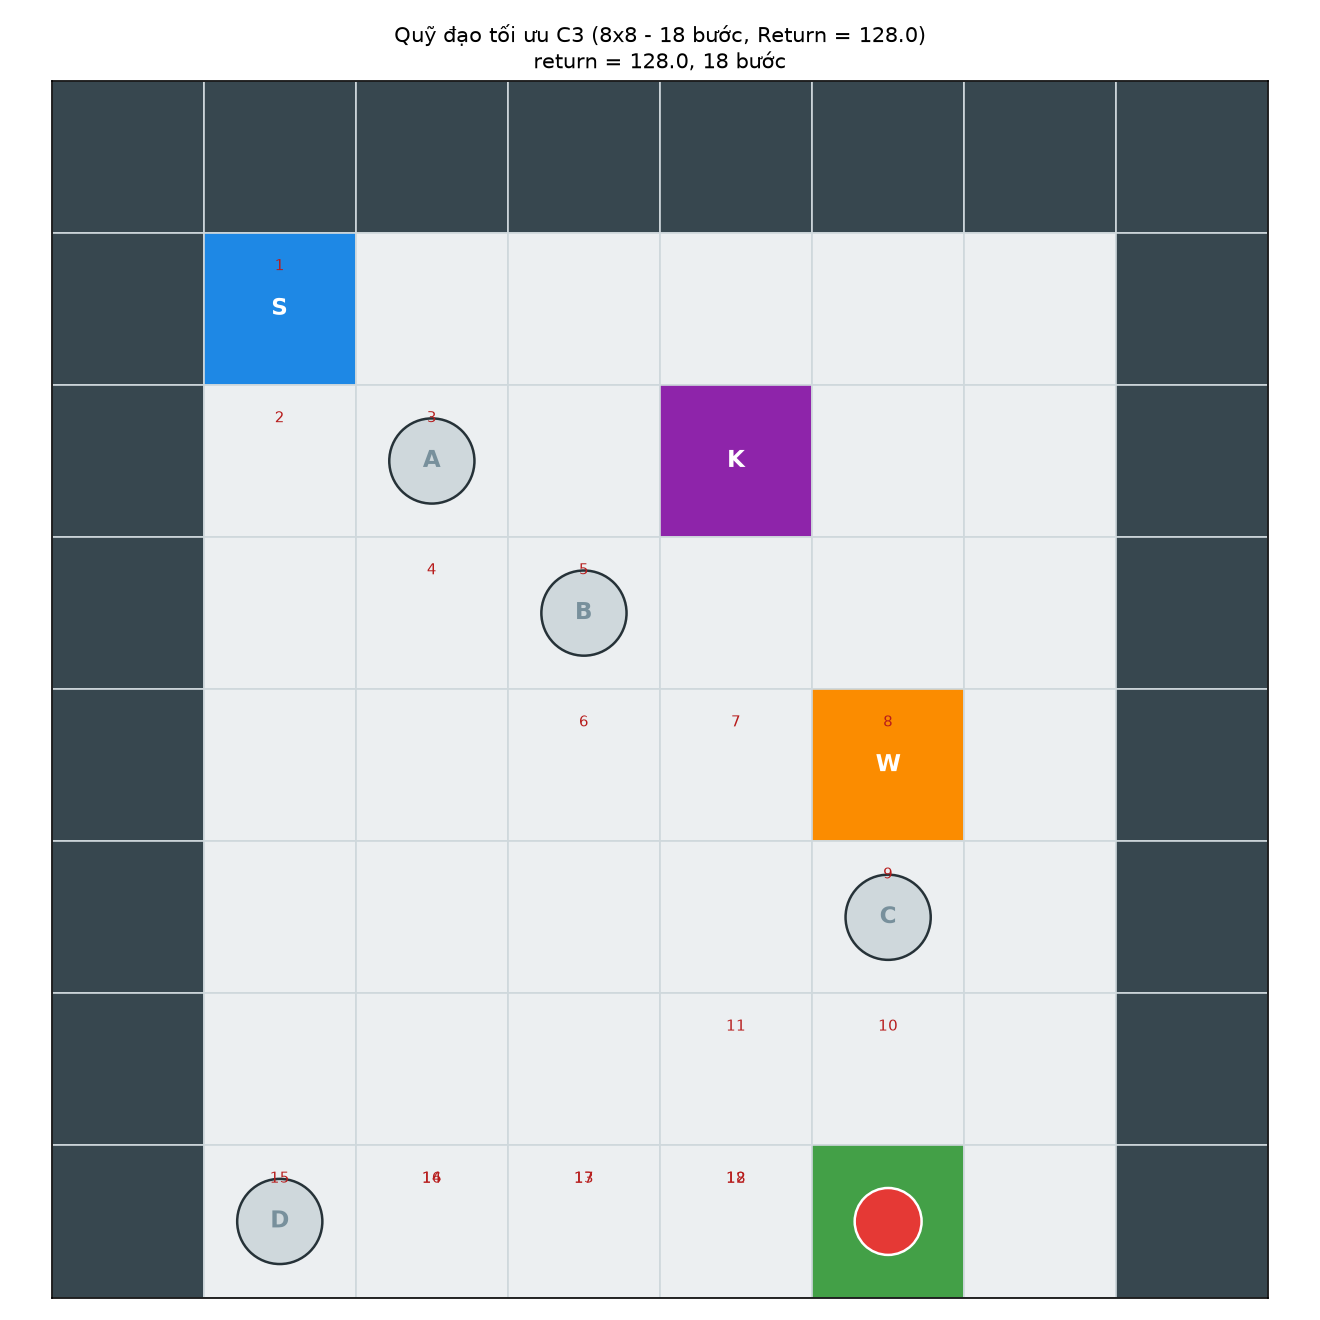
\includegraphics[width=0.31\textwidth]{figures/policy_C3_Hard_8x8.png}
\caption{Learned greedy policy arrows across the three benchmark environments: Level 1 (left), Level 2 (middle), and Level 3 (right).}
\label{fig:policies}
\end{figure*}

\subsection{Reward Formulation Sensitivity Analysis}
To evaluate the impact of reward shaping, we altered the step penalty $r_{\text{step}}$ on Level 3 across three distinct profiles (Table~\ref{tab:reward_ablation} and Fig.~\ref{fig:reward_exp}):
\begin{itemize}
    \item \textbf{Cheap Steps ($r_{\text{step}} = -0.2$):} Step costs are minimal. Collecting all four items ($+40.0$ target rewards) clearly outweighs step penalties. The optimal policy takes 18 steps and does not use the skip tile, achieving a return of $+137.6$. Q-Learning converges to this exact policy.
    \item \textbf{Default Steps ($r_{\text{step}} = -1.0$):} Standard baseline. Collecting all four items earns $+128.0$ (18 steps), while skipping an item earns $+120.0$ (14 to 18 steps).
    \item \textbf{Expensive Steps ($r_{\text{step}} = -5.0$):} Step penalties are severe. Traveling to switch $W$ and item $C$ incurs high step costs. Skipping an item to reach the exit earlier becomes the mathematically optimal strategy, earning $+80.0$ with skip tile used. Q-Learning correctly adopts the shortcut.
\end{itemize}

\begin{table}[htbp]
\caption{Reward Sensitivity Experiment on Level 3 ($8\times 8$)}
\label{tab:reward_ablation}
\centering
\begin{tabular}{lcccc}
\toprule
\textbf{Step Cost Profile} & $r_{\text{step}}$ & \textbf{Optimal Return} & \textbf{Learned Return} & \textbf{Skip Used} \\
\midrule
Cheap Steps     & $-0.2$ & $+137.6$ & $+137.6$ & No \\
Default Steps   & $-1.0$ & $+128.0$ & $+120.0$ & Yes \\
Expensive Steps & $-5.0$ & $+80.0$  & $+80.0$  & Yes \\
\bottomrule
\end{tabular}
\end{table}

\begin{figure}[htbp]
\centering
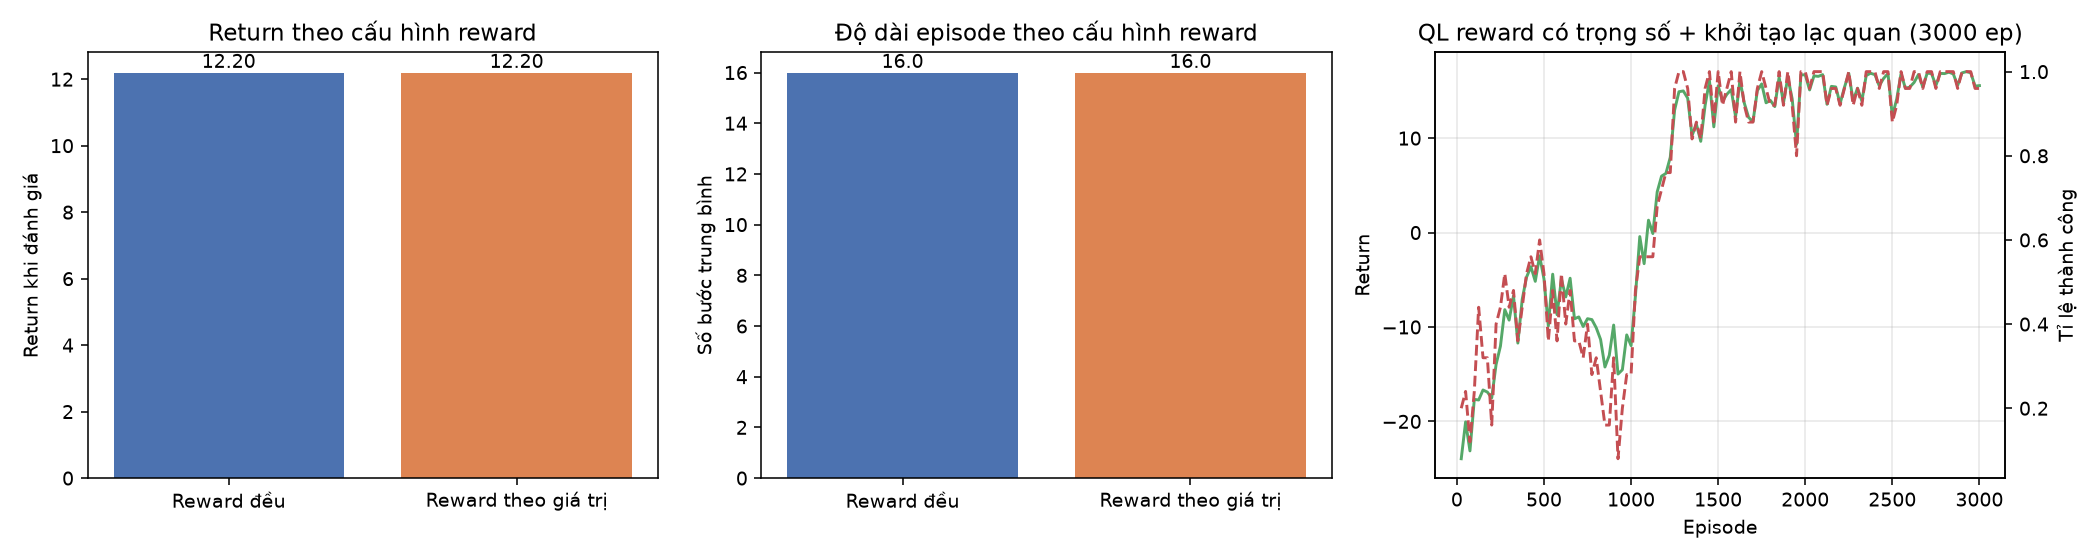
\includegraphics[width=0.48\textwidth]{figures/reward_experiment.png}
\caption{Comparison of learned returns on Level 3 under cheap ($-0.2$), default ($-1.0$), and expensive ($-5.0$) step penalties.}
\label{fig:reward_exp}
\end{figure}

\subsection{Seed Sensitivity and Local Optima on Level 3}
Level 3 features a bonus skip tile $K$ placed near item $A$. Using $K$ advances progress immediately, allowing the agent to skip collecting one item. Taking the shortcut yields $+120.0$, whereas completing the full 4-item sequence earns $+128.0$. Because the shortcut is encountered early during random exploration, agents can be trapped in this local optimum.

We evaluated Policy Iteration, Q-Learning, SARSA, and Monte Carlo across three independent seeds ($\{42, 7, 123\}$) on Level 3 (Table~\ref{tab:seed_exp}):
\begin{itemize}
    \item Policy Iteration consistently achieves the global optimum $+128.0$ without skip tile across all seeds.
    \item Q-Learning escapes the local optimum in 2 out of 3 seeds (seed 7 and seed 123), reaching $+128.0$. In seed 42, it takes the shortcut ($+120.0$).
    \item SARSA is trapped in the local optimum across all three seeds ($+120.0$, skip used = True).
    \item Monte Carlo is also trapped across all three seeds ($+118.0$ to $+119.0$, skip used = True).
\end{itemize}

\begin{table}[htbp]
\caption{Multi-Seed Evaluation on Level 3 ($8\times 8$)}
\label{tab:seed_exp}
\centering
\begin{tabular}{lcccc}
\toprule
\textbf{Algorithm} & \textbf{Seed 42} & \textbf{Seed 7} & \textbf{Seed 123} & \textbf{Shortcut Trap Rate} \\
\midrule
Policy Iteration & $+128.0$ & $+128.0$ & $+128.0$ & 0 / 3 (0\%) \\
Q-Learning       & $+120.0$ & $+128.0$ & $+128.0$ & 1 / 3 (33\%) \\
SARSA            & $+120.0$ & $+120.0$ & $+120.0$ & 3 / 3 (100\%) \\
Monte Carlo      & $+119.0$ & $+118.0$ & $+119.0$ & 3 / 3 (100\%) \\
\bottomrule
\end{tabular}
\end{table}

\subsection{Learning Rate Sensitivity Analysis}
Fig.~\ref{fig:alpha_sens} displays training performance under four learning rates $\alpha \in \{0.01, 0.05, 0.10, 0.20\}$. When $\alpha = 0.01$, learning progress is slow. Intermediate values $\alpha = 0.05$ and $\alpha = 0.10$ exhibit smooth, reliable convergence. When $\alpha = 0.20$, early training exhibits oscillations before stabilizing.

\begin{figure}[htbp]
\centering
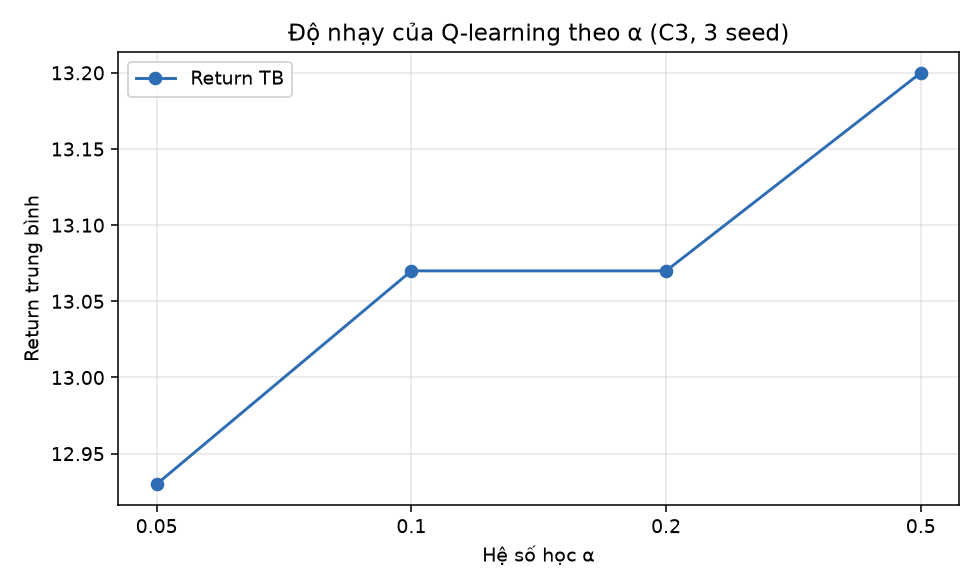
\includegraphics[width=0.48\textwidth]{figures/alpha_sensitivity.png}
\caption{Sensitivity analysis of learning rate $\alpha \in \{0.01, 0.05, 0.10, 0.20\}$ on training return convergence.}
\label{fig:alpha_sens}
\end{figure}

\section{Discussion}

\subsection{State Augmentation and Markov Compliance}
Our results confirm that explicit state augmentation successfully resolves the non-Markovian challenge. By including progress $p$, switch state $w$, and skip token $tok$, the state space grows from 49 spatial cells to 693 discrete states on Level 3. This size is completely tractable for tabular representations, allowing exact Bellman optimality computation without function approximation.

\subsection{On-Policy versus Off-Policy Exploration Dynamics}
The multi-seed experiment provides clear insight into algorithm exploration behavior. Q-learning uses an off-policy update with $\max_{a'} Q(s', a')$. Once exploration uncovers the $+10.0$ bonus from item $C$, the Bellman optimality backup rapidly propagates this high value back through the chain, allowing Q-Learning to switch from the shortcut to the full sequence.

In contrast, on-policy SARSA updates values based on the actions actually chosen by its $\epsilon$-greedy policy. Exploratory actions occasionally bump into locked cells or walls, which incur penalties. As a result, SARSA assigns lower values to the longer path, reinforcing its preference for the safer shortcut.

\subsection{Monte Carlo Control Variance and Convergence}
Monte Carlo control requires complete episode rollouts before updating values. Because early rollouts take random walks with wide variance in total returns, MC updates exhibit substantial noise. While MC achieves 100\% task completion after 20,000 episodes, its convergence rate is slower than temporal difference methods.

\subsection{Reward Design Insights}
The experiment confirms two important reward design principles:
\begin{enumerate}
    \item \textbf{Early-Exit Penalty Necessity:} Setting $r_{\text{early}} = -20.0$ is essential. Without this negative penalty, agents learn to exit immediately to minimize step costs.
    \item \textbf{Step Cost Sensitivity:} The ratio between step penalty $r_{\text{step}}$ and item bonus $r_{\text{collect}}$ directly dictates whether agents take shortcuts. Rational RL policies adapt their trajectory length based on step penalties.
\end{enumerate}

\subsection{Limitations}
The primary limitation of tabular RL is scalability. In an $M \times N$ grid with $K$ sequential items and auxiliary mechanisms, the potential state space scales as $\mathcal{O}(M \times N \times 2^K)$. For large maps or long target sequences, deep reinforcement learning with neural network function approximation would be necessary.

\section{Conclusion}
In this project, we solved the Ordered Treasure Hunt benchmark using tabular reinforcement learning. We designed an augmented state representation that strictly preserves the Markov property. Across three square gridworld maps ($5\times 5$, $7\times 7$, and $8\times 8$), all five algorithms---Value Iteration, Policy Iteration, Q-Learning, SARSA, and Monte Carlo Control---achieved a 100\% mission success rate. Model-based dynamic programming provided exact analytical baselines. Q-Learning successfully escaped shortcut local optima on the hard map in 2 out of 3 seeds, whereas on-policy algorithms favored the shortcut. Finally, step penalty variations confirmed that the optimal policy shifts rationally between shortcuts and full sequence collection based on step costs.

\section*{Acknowledgment}
The author thanks the Faculty of Electrical and Electronic Engineering at Phenikaa University for providing computing resources and academic guidance throughout this coursework project.

\begin{thebibliography}{00}
\bibitem{sutton2018reinforcement}
R.~S. Sutton and A.~G. Barto, \emph{Reinforcement Learning: An Introduction}, 2nd~ed. Cambridge, MA, USA: MIT Press, 2018.

\bibitem{watkins1992q}
C.~J. Watkins and P.~Dayan, ``Q-learning,'' \emph{Machine Learning}, vol.~8, no.~3--4, pp.~279--292, 1992.

\bibitem{rummery1994line}
G.~A. Rummery and M.~Niranjan, ``On-line Q-learning using connectionist systems,'' Cambridge Univ. Eng. Dept., Tech. Rep. CUED/F-INFENG/TR 166, 1994.

\bibitem{bertsekas2012dynamic}
D.~P. Bertsekas, \emph{Dynamic Programming and Optimal Control}, 4th~ed. Belmont, MA, USA: Athena Scientific, 2012.

\bibitem{bellman1957dynamic}
R.~Bellman, ``A Markovian decision process,'' \emph{Journal of Mathematics and Mechanics}, vol.~6, no.~5, pp.~679--684, 1957.

\bibitem{mnih2015human}
V.~Mnih et~al., ``Human-level control through deep reinforcement learning,'' \emph{Nature}, vol.~518, no.~7540, pp.~529--533, 2015.

\bibitem{culberson1997sokoban}
J.~C. Culberson, ``Sokoban is PSPACE-complete,'' Tech. Rep. TR 97-02, Dept. Comput. Sci., Univ. Alberta, 1997.
\end{thebibliography}

\end{document}
